\documentclass[10pt,oneside]{report}

% Encoding and font packages
\usepackage[table]{xcolor}
\usepackage[utf8]{inputenc}
\usepackage[T1]{fontenc}
\usepackage{lmodern}
\usepackage{booktabs}
\usepackage[nottoc]{tocbibind} % If you don't want the main TOC itself listed
\usepackage{setspace}
\onehalfspacing
\usepackage{hyperref}
\hypersetup{
    colorlinks=true,
    linkcolor=blue,
    filecolor=magenta,      
    urlcolor=cyan,
    citecolor=blue
}
\usepackage[numbers]{natbib}
\usepackage[colorinlistoftodos,prependcaption,textsize=small]{todonotes}
\usepackage{adjustbox}
\usepackage{graphicx}
\graphicspath{ {./images/} }
\usepackage{subcaption}

\usepackage{anyfontsize}
\usepackage{lmodern}
% Dynamically scale font sizes (80% of original)
\let\oldnormalsize\normalsize
\renewcommand{\normalsize}{\fontsize{8}{10}\selectfont}
\let\oldlarge\large
\renewcommand{\large}{\fontsize{10}{12}\selectfont}
\let\oldLarge\Large
\renewcommand{\Large}{\fontsize{11.5}{13.8}\selectfont}
\let\oldLARGE\LARGE
\renewcommand{\LARGE}{\fontsize{13}{15.6}\selectfont}
\let\oldhuge\huge
\renewcommand{\huge}{\fontsize{16}{19.2}\selectfont}
\let\oldHuge\Huge
\renewcommand{\Huge}{\fontsize{20}{24}\selectfont}

% Begin document
\begin{document}

% -------------------------
% Title Page
% -------------------------
\begin{titlepage}
    \centering
    % Title (two lines)
    {\LARGE TODO TITLE\\\par}
    \vspace{2cm}
    % Subtitle/description
    {\large A report submitted to the University of Manchester for the degree of
    Bachelor of Science in the Faculty of Science and Engineering\par}
    \vspace{2cm}
    \vspace{1cm}

    {\large Author: Sai Putravu\par}
    {\large Student id: 10829976\par}
    {\large Supervisor: TODO\par}
    \vfill
    % Department
    % Date
    {\large 2025\par}
    \vspace{1cm}
    {\large School of Computer Science\par}
\end{titlepage}

% Roman page numbering for preliminary pages
\pagenumbering{roman}

% -------------------------
% Table of Contents
% -------------------------
\tableofcontents
\clearpage

% -------------------------
% List of Figures
% -------------------------
\listoffigures
\clearpage

% -------------------------
% List of Tables
% -------------------------
\listoftables
\clearpage


% -------------------------
% Abbreviations and Acronyms
% -------------------------
% \phantomsection
\addcontentsline{toc}{chapter}{Abbreviations and Acronyms}
\chapter*{Abbreviations and Acronyms}

\todo{Alphabetically sort this}
\begin{table}[ht]
    \centering
    \begin{tabular}{ll}

        \textbf{BERT} & Bidirectional Encoder Representation from Transformers. \\
        \textbf{CBM} & Condition-based maintenance policy. \\
        \textbf{CNN} & Convolutional Neural Network. \\
        \textbf{DBSCAN} & Density-Based Spatial Clustering of Application with Noise. \\
        \textbf{DL} & Deep Learning. \\
        \textbf{EPB1} & Extracted proton beam line 1. \\
        \textbf{EPB2} & Extracted proton beam line 2. \\
        \textbf{ELMo} & Embeddings from Language Models. \\
        \textbf{FLD} & First-line diagnosis system. \\
        \textbf{GPT} & Generative Pre-trained Transformer. \\
        \textbf{HDBSCAN} & Hierarchical Density-Based Spatial Clustering of Application with Noise. \\
        \textbf{HDD} & Hard-Disk Drive. \\
        \textbf{HEDS} & High energy drift space. \\
        \textbf{IoT} & Internet of Things. \\
        \textbf{LEBT} & Low energy beam transport line. \\
        \textbf{LINAC} & Linear Accelerator. \\
        \textbf{FAP} & Fault Analysis Pathway. \\
        \textbf{LSA} & Latent Semantic Analysis. \\
        \textbf{ML} & Machine Learning. \\
        \textbf{NLP} & Natural Language Processing. \\
        \textbf{PCA} & Principle Component Analysis. \\
        \textbf{PdM} & Predictive maintenance policy. \\
        \textbf{PLM} & Pre-trained Language Model. \\
        \textbf{PvM} & Preventative maintenance policy. \\
        \textbf{R2F} & Run-to-failure maintenance policy. \\
        \textbf{RFQ} & Radio-frequency quadrupole. \\
        \textbf{RF} & Random Forest. \\
        \textbf{SAFE} & Supervised Aggregative Feature Extraction. \\
        \textbf{SMART} & Self-monitoring and reporting technology. \\
        \textbf{STFC} & Science and Technology Facilities Council. \\
        \textbf{SVD} & Singular Value Decomposition. \\
        \textbf{SVM} & Support Vector Machine. \\
        \textbf{TS-1} & Target Station 1. \\
        \textbf{TS-2} & Target Station 2. \\
        \textbf{t-SNE} & t-distributed Stochastic Neighbour Embedding. \\
        \textbf{UKRI} & United Kingdom Research and Innovation. \\
        \textbf{UMAP} & Uniform Manifold Approximation and Projection. \\
        \textbf{MCR} & Main Control Room. \\
        \textbf{Operalog} & The ISIS Operational Log. \\

    \end{tabular}
\end{table}

\clearpage

% Switch to Arabic numbering after preliminary pages
\pagenumbering{arabic}

% -------------------------
% Chapters
% -------------------------
\chapter*{Abstract}
\todo[inline]{TODO}


\chapter{Introduction}

This project concerns the use of statistical and Machine Learning models to augment the predictive maintenance process at the STFC Rutherford Appleton Laboratory's ISIS Neutron and Muon research facility. The ISIS Neutron and Muon facility is a research centre for physical and life sciences, owned and operated by the STFC, a council that forms the UK Research and Innovation. In order to produce beams of neutrons and muons, allowing scientists to study materials at the atomic level, large and complex structures and machinery are required. The facility has a wealth of instrumentation taking multitudes of measurements to ensure that proper maintenance is completed in a timely manner. \\

\todo[inline] {Finish this off}
\textbf{ }
\todo[inline,caption={}]{
Introduce the sections of the paper.
\begin{itemize}
    \item Refine this after coming back
    \item Section 2,
    \item Section 3, 
    \item ...
\end{itemize}
}


\section{Motivation}
Motivate the research project.


\todo[inline,caption={}]{
The things in this section will include
\begin{itemize}
    \item Introduce the problem: Auto-categorisation and label inference
    \item Highlight the research aims. This should highlight the vastly open nature of the project and then hone in on the particular issue I am tackling. (i.e. to progress the state of PdM ...)
    \item Identify the data input, expected output, data shape and explain why this motivates the project
\end{itemize}
}


\section{Overview of the ISIS Research Facility}\label{sec:isisbg}

The STFC Rutherford Appleton Laboratory's ISIS Neutron and Muon research facility is a research centre for physical and life sciences. It is owned and operated by the STFC, a council within the United Kingdom Research and Innovation (UKRI). The UKRI is a public body of the United Kingdom's Government that directs funding for research and innovation through the science budget of the Department for Science, Innovation and Technology. ISIS was designed in the 1970s and early 1980s, with the core of the design being a strong-focusing machine with six radio frequency accelerating cavities to provide an average beam current of $200\mu A$ \cite{thomason2019isis}. According to (\citet{thomason2019isis}), with the introduction of ISIS and other neutron sources, rapid development of neutron instrumentation was stimulated. Over the years, the facility has been augmented with numerous components and instruments, such as the second target station - the current schematic representation of the facility can be seen in Figure~\ref{fig:isis}.

\begin{figure}[htbp]
    \centering
    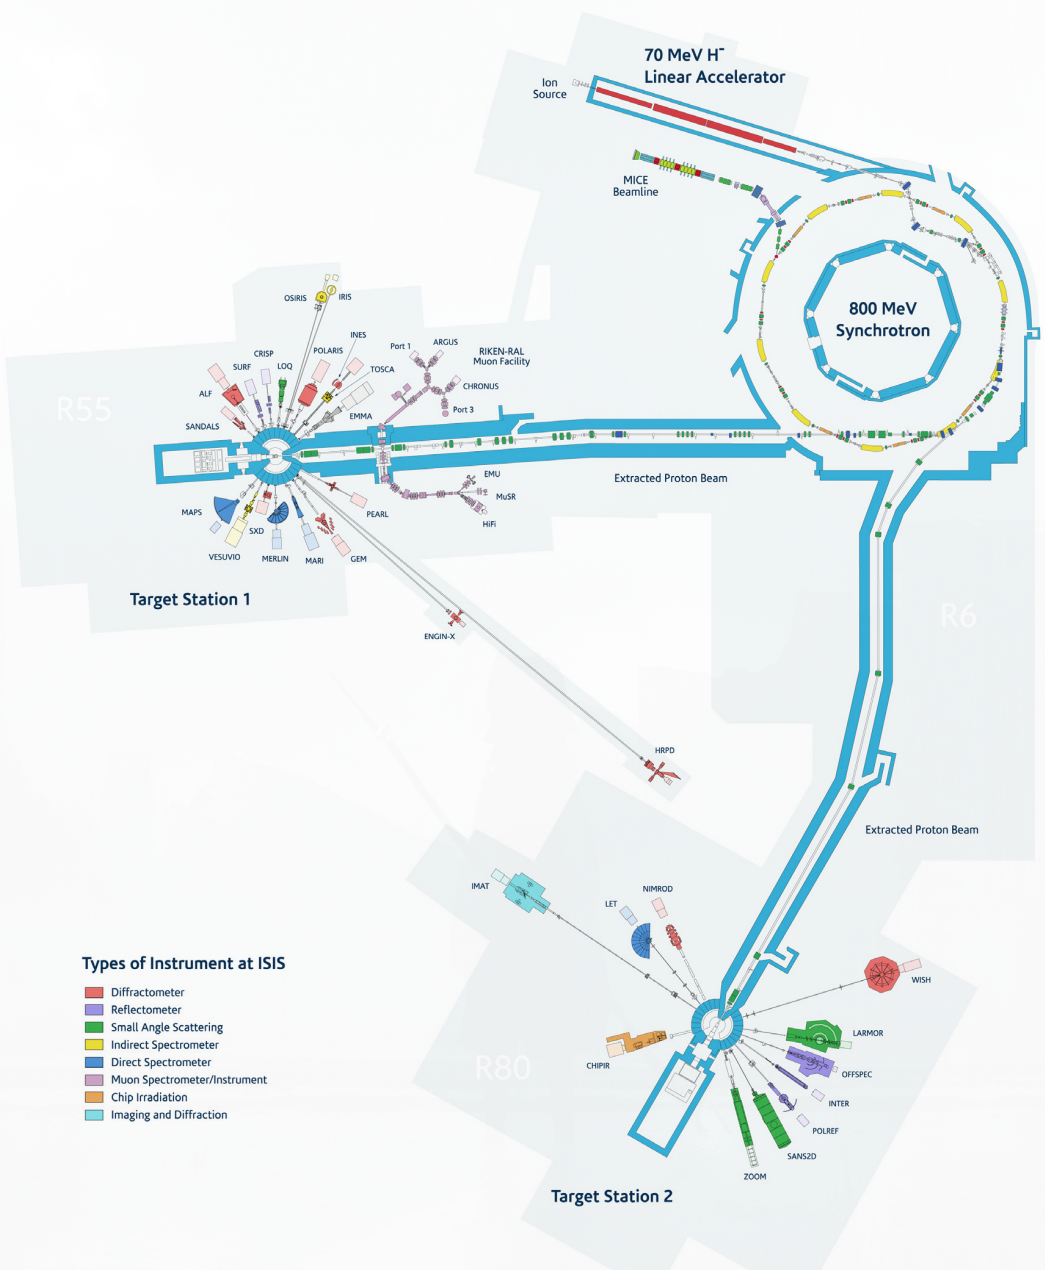
\includegraphics[width=0.95\textwidth]{ISIS.png}
    \caption{The schematic representation of the physical layout of ISIS. The light grey areas are footprints of the buildings. Source: (\citet{thomason2019isis}).}\label{fig:isis}
\end{figure}

\subsection{The end-to-end production of neutrons and muons}
\begin{figure}[htbp]
    \centering
    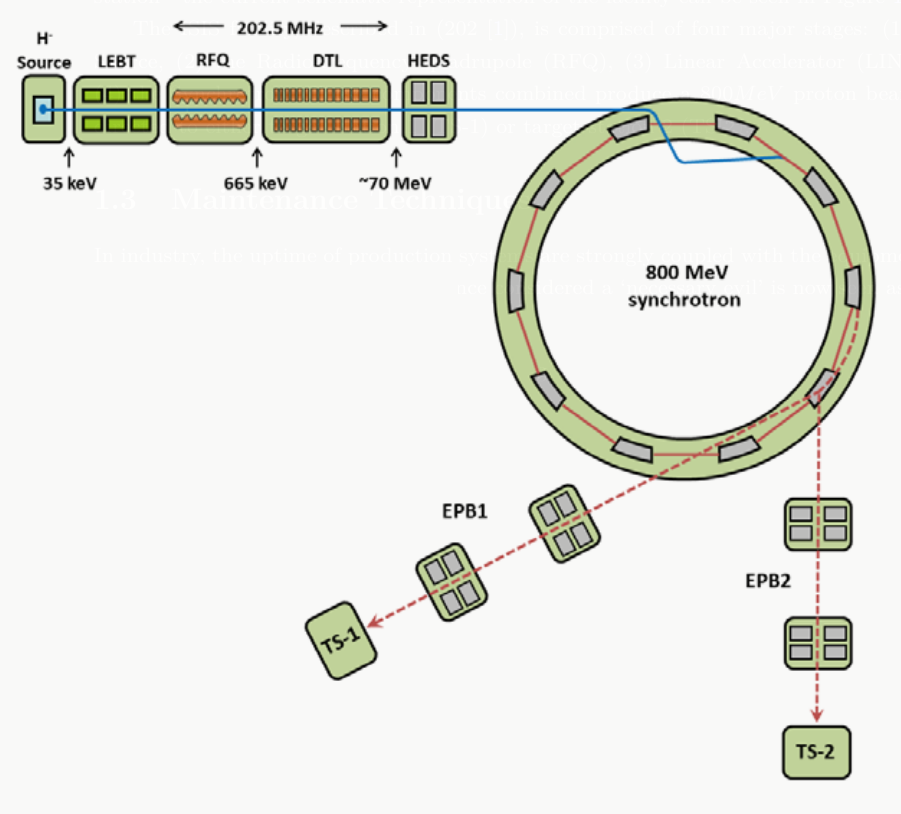
\includegraphics[width=0.6\textwidth]{ISIS2.png}
    \caption{ISIS ion source and chain of accelerators, with $H^-$ ions in blue and protons in red. Not to scale. Source: (\citet{2021practicalguide}).}\label{fig:isis2}
\end{figure}

The ISIS facility, described in A Practical Guide to the ISIS Neutron and Muon Source (\citet{2021practicalguide}), is comprised of four major stages: (1) the ion source, (2) the radio-frequency quadrupole (RFQ), (3) linear accelerator (LINAC) and (4) the synchrotron. These components combine to produce a 800 MeV proton beam that is directed to either target station 1 (TS-1) or target station 2 (TS-2). Starting with $H^-$ ions (protons with two orbiting electrons), the path taken through the four stages is shown in Figure~\ref{fig:isis2}. Throughout the entire $H^-$ or proton acceleration process, the beam must be kept under good vacuum and, to do so, many tens of vacuum pumps are maintaining the vacuum between $10^{-8}$ and $10^{-9}$ of atmospheric pressure.

The first stage of the ISIS machine is the ion source, which generates the negative hydrogen ($H^-$) ions, which are then accelerated through the RFQ and LINAC. This ion source is a pulsed source that ionises hydrogen gas via an electric discharge between an internal anode and cathode \cite{2021practicalguide}. As detailed in the guide, around 20ml of hydrogen gas per minute is continuously delivered to the ion source from a hydrogen gas bottle. Once the $H^-$ ions emerge from the ion source, they have an energy of 35 keV and are presented to the RFQ via the Low Energy Beam Transport line (LEBT). The LEBT prevents the low-energy $H^-$ beam from increasing in size (due to the mutual repulsion of the ions) and also incorporates a beam stop. This is essentially a remotely removable sheet of metal that physically blocks the beam.

Following the ion source and LEBT, the $H^-$ beam enters the RFQ. This section of the machine utilises high-intensity radio frequency electric fields that contain (focus), group (bunch) and begin accelerating the particles in this beam up to an energy of 665 keV. A key function of the RFQ is to isolate downstream accelerators from variations originating in the ion source, thereby improving beam stability in the LINAC, synchrotron and target stations \cite{2021practicalguide}. 

The subsequent stage is the LINAC, which increases the beam energy from 665 keV to 70 MeV. This acceleration is achieved via high-intensity radio-frequency fields arranged in structure to possess a very high Q factor \cite{michael2006electronic} (around 50,000). This means their geometry must be exceptionally stable. Through the precise temperature regulation of the cooling water tank, ensuring it is significantly under $1^\circ C$, the effects of thermal expansion and contraction are countered \cite{2021practicalguide}. Furthermore, maintaining a high vacuum is critical throughout the LINAC. Failure to do so can lead to premature stripping of loosely bound electrons in the $H^-$ ions, consequently leading to an increase in radioactivity and particle loss (i.e. beam loss). To detect and warn about such cases, beam loss monitors are installed throughout the LINAC, which provide indicate whenever there is an excessive loss in particles. \cite{2021practicalguide}.

Once the $H^-$ particles leave the LINAC, they then pass through a beam transport line - the High Energy Drift Space (HEDS). The function of this is to mainly reduce the particles spreading and focus the beam to the synchrotron. To accumulate the high intensity beam in the synchrotron, ISIS employs charge-exchange injection . This technique allows incoming $H^-$ beam from the LINAC to be `layered' into the synchrotron's circumference over many turns. As the $H^-$ ions enter the synchrotron ring, they pass through a thin foil which strips away their two electrons, converting them to protons. The charge-exchange injection process is specifically chosen as it is the most efficient way of taking and wrapping a long string of particles around the circumference of a synchrotron \cite{2021practicalguide, ankenbrandt1980h}.

The 70 MeV beam is then injected into the synchrotron, which is the primary accelerator ring at ISIS. This ring boosts the (now proton) beam energy to 800 MeV. For an idea of scale, the machine has a circumference of around 163m (corresponding to a radius of approximately 26m). It features a repeating structure of ten `superperiods'. Each superperoid uses dipole magnets to bend the proton path by $36^\circ$ and quadrupole magnets to maintain beam focus \cite{2021practicalguide}. The protons gain energy over just under 8000 revolutions, as each turn gives a proton 0.1 MeV. While the protons gain energy, the magnetic fields and accelerating radio-frequency voltages must be, very precisely, increased in synchronism. The initially continuous ring of injected protons is gathered into two distinct bunches, a little more than $0.1\mu s$ apart, using a low-level radio-frequency voltage before the main acceleration begins \cite{2021practicalguide}.

Once accelerated, in order to direct the proton bunches towards a pre-selected target station (TS-1 or TS-2) three kicker magnets are used which deflect the bunches upwards. These bunches are then bent into the respective extracted proton beam lines (EPB1 or EPB2). These transfer lines utilise magnets to steer the beam towards the respective target stations. Additionally, as a safety precaution, both lines are heavily shielded in thick steel and concrete and beam loss monitors are installed along their length to detect any errant particles \cite{2021practicalguide}.

The primary purpose of the ISIS facility culminates at the target stations. The high-energy proton beam collides with a dense, high atomic number target (tantalum-clad tungsten at ISIS) designed to produce a large number of neutrons via spallation, within a compact region of space \cite{2021practicalguide}. These energetic neutrons are then slowed down (moderated) by surrounding materials (liquid nitrogen, liquid hydrogen and water at ISIS) and reflected back towards instruments by a beryllium reflected \cite{sharma2001nuclear, 2021practicalguide}. Additionally, ISIS produces muons for experiments by inserting a thin (roughly 1cm thick) graphite target into the proton beam around 20m away from the TS-1 neutron target. Collision in this target generates pions, which subsequently decay into muons \cite{2021practicalguide}.

\noindent This detailed description sourced from the guide highlights some key takeaways. There are an incredible number of points of failure in the facility due to the highly precise and radioactive nature of the task. The ISIS team has taken many precautions such as fault detection mechanisms (i.e. the beam loss monitors), breakdown counter-measures (i.e. the thick layer of steel and concrete in the EPB1 and EPB2 lines). However, as there are a large number of components that can go wrong and issues that may arise, regular maintenance is required. 

\subsection{Maintenance at ISIS} 
As detailed in the 33-year historical account of the ISIS facility (\citet{thomason2019isis}), the ISIS operations occur in cycles, periods of roughly 30-50 days where the machine runs constantly without breaks. Roughly 10 days before the scheduled start of a cycle, and gaps between cycles typically range from 1 week to 3 months. In addition, typically every four years, shutdowns scheduled for 6-9 months occur for major maintenance and upgrade work. On the ground, day-to-day operations are run from the Main Control Room (MCR) by the ISIS crew which consists of 6 shift teams of the following roles: (1) duty officer, (2) assistant duty officer and (3) duty technician. \todo{Add the graph, if you can ever figure out the operating cycles before 2016.} The expertise and rapid response capabilities of these trained operational crews are vital for both routine operation and initial fault response.
Minimising this downtime is crucial for several reasons inherent to operating a large-scale user facility like ISIS \cite{thomason2019isis}. Primarily, unscheduled downtime directly impacts the international researchers allocated beam time, potentially jeopardising experiments planned months or years in advance and wasting valuable research opportunities. Furthermore, interruptions disrupt the tightly packed operational schedule, reduce the overall scientific output, and incur significant operational costs without delivering the facility's core research product \cite{thomason2019isis}. Therefore, understanding the factors that contribute to downtime and implementing strategies to mitigate it are paramount.
Many factors affect downtime such as having a robust plan, the day-to-day operators' knowledge of the system and adequate inventories of spares \cite{thomason2019isis}. Figure~\ref{fig:isisDowntime} shows the ratio of downtime to active machine operation since 2016, with over half the time of the machine since 2016 being down. In other words, over half the time, the machine is not active and is undergoing maintenance. This highlights the trade-off between maximising operational availability and minimizing failures through planned maintenance. The major maintenance strategies and their trade-offs are further explored in Section~\ref{sec:maintenanceTechniques}.

To help reduce downtime, over the last few years, a first-line diagnosis (FLD) system was introduced, presented in (\citet{fld2017}). The FLD system helps reduce downtime by providing expert guidance on fault diagnosis and resolution, which has been shown to improve the dissemination of knowledge from experts to operations. The FLD utilises Fault Analysis Pathways (FAPs), which provide structural links between ISIS subsystems. This allows users of the system to access granular subsystems' local documentation minimising file hunting and saving time and effort. An example FAP can be seen in Figure~\ref{fig:fap}.

\begin{figure}[htbp]
    \centering
    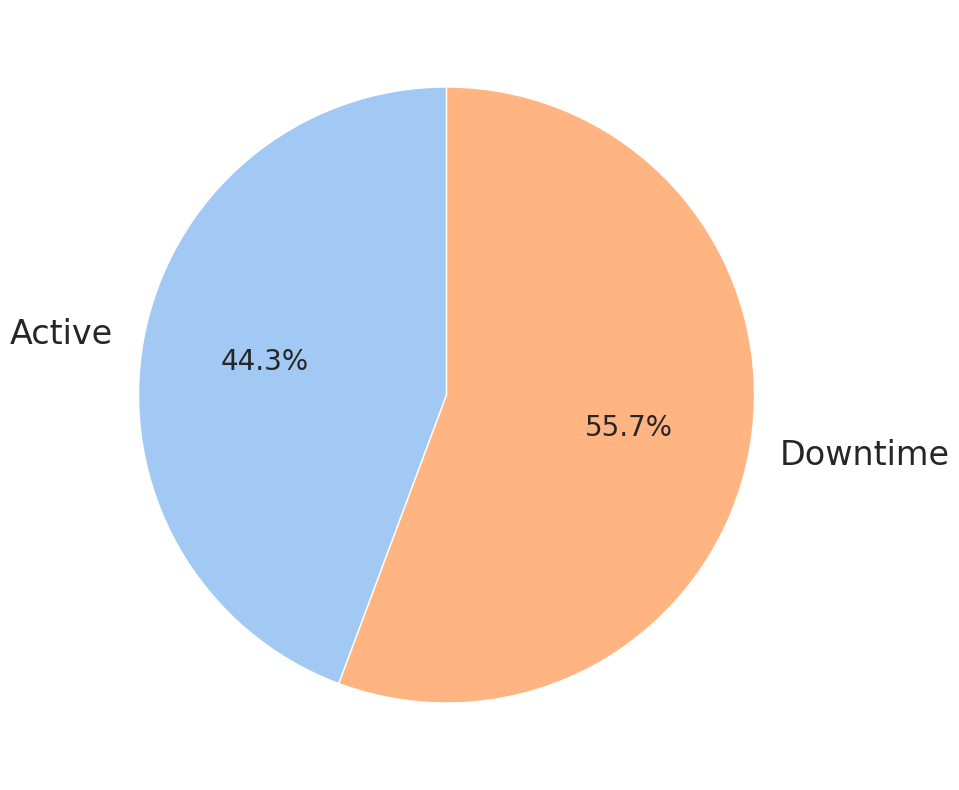
\includegraphics[width=0.5\textwidth]{isisDowntime.png}
    \caption{A visualisation of the machine downtime as opposed to time operating, according to the ISIS operational cycle. Data source: (\citet{isisbeamoperations2024})}\label{fig:isisDowntime}
\end{figure}
\begin{figure}[htbp]
    \centering
    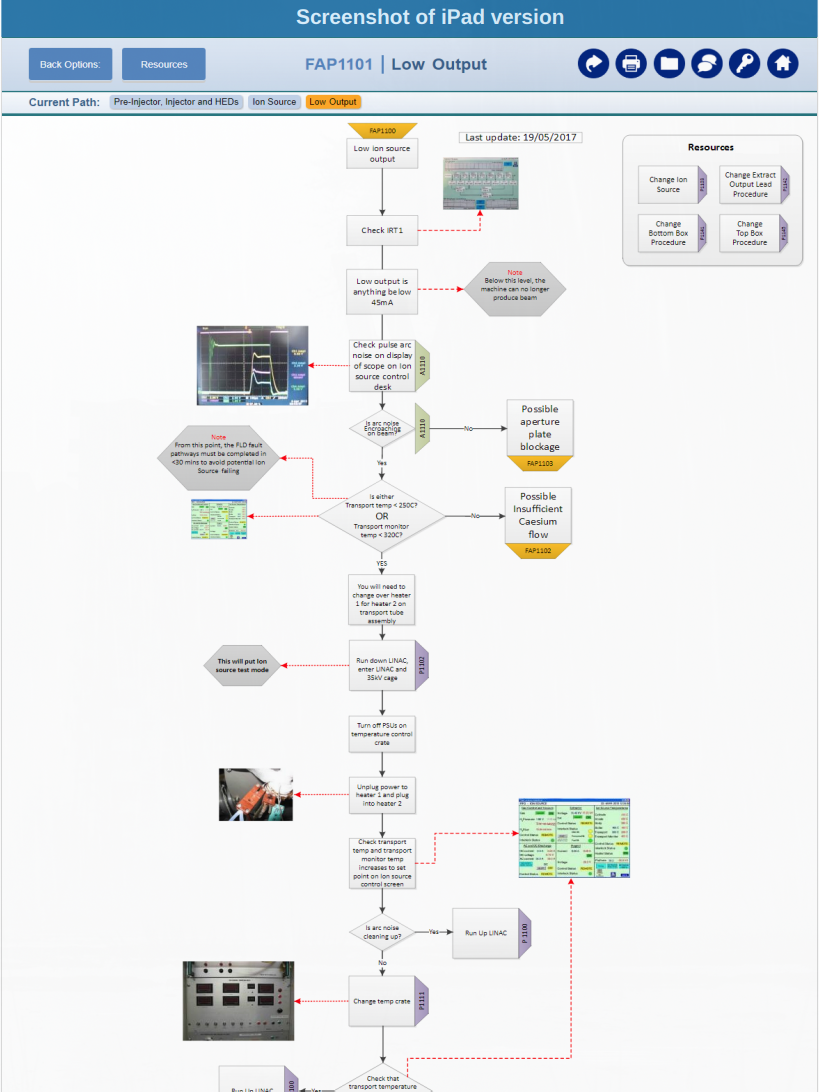
\includegraphics[width=0.95\textwidth]{fap.png}
    \caption{Example FAP1101, screenshotted from an iPAD version of FLD version 2.2, which shows the FAP for pre-injector, injector and High Energy Drift Space. Source: (\citet{fld2017})}\label{fig:fap}
\end{figure}


\textbf{}\\
\todo[inline,caption={}]{
Introduce the research topic. 
The things in this section will include
\begin{itemize}
    \item Talk about the ISIS research facility - DONE
    \item Talk about the Operational Cycle for ISIS - SORT OF DONE (graph too)
    \item Talk about the ISIS Crew and importance of having trained staff on premises. - SORT OF
    \item Talk about the Lost time and why it is important to minimise this for the ISIS research facility. - SORT OF
    \item Describe the first-line diagnosis system (FLD) and FAPs. - DONE
    \item Talk about the Datasets, operalog (MOVED)
\end{itemize}
}


\section{Maintenance Techniques}\label{sec:maintenanceTechniques}
In industry, the uptime of production systems are strongly coupled with the equipment maintenance. So much so that what was once considered a `necessary evil' is now seen as a `profit contributor' to be able to maintain a competitive edge \cite{waeyenbergh2002framework, faccio2014industrial}. For facilities aiming to provide systems for research, maintenance impacts the downtime and cost of running. As a result, both to minimise unexpected downtime and provide a competitive edge, many industrial applications collect vast quantities of data during the entire life cycle of the system. This large amount of data may include information about processes, events and alarms \cite{carvalho2019systematic} which occur along the industrial production line, collected by different equipment. The equipment may be located in different locations in the sub-components of the larger system or even different sub-components themselves. \todo{talk about maintenance itself in a lot more depth}

In the literature, various terms and categories of maintenance arise each with differing strategies \cite{susto2012predictive, mobley2002introduction, susto2016dealing}. Thus, while there exists some disagreement in nomenclature, we consider the four categories presented in (\citet{susto2012predictive}). The four maintenance policy categories are as follows, noting that each policy has, uniquely, their own benefits and drawbacks:

\begin{enumerate}
    \item{Run-to-failure (R2F) maintenance: Continual usage of the system until failure. Restoration is performed at the point of noticing failure condition. This is the simplest approach and typically the most costly method as it reduces the facility's availability and requires a complete replacement of parts.} 
    \item{Preventative maintenance (PvM): Otherwise referred to as scheduled maintenance, performing maintenance at regular intervals to increase longevity of the component or in anticipation of the end of expected life of the component. While this typically prevents many errors, it wastes maintenance cycles when systems are perfectly healthy. Hence, causing unnecessary downtime and cost.}
    \item{Condition-based maintenance (CBM): Taking the action to perform maintenance on equipment through monitoring various health characteristics and metrics of the components of the system. This approach requires continuous monitoring and, thus, allows for close to instant response on maintenance only when required. However, a drawback of this policy is that one cannot plan maintenances in advance.}
    \item{Predictive maintenance (PdM): Otherwise referred to as statistical-based maintenance, only performs maintenance actions when determined necessary. Prediction tools are utilised to implement forward-planning and scheduling systems, using statistical inference methods. However, if these statistical inferences are not accurate, the whole system suffers which inevitably leads to additional downtime and costs.}
\end{enumerate}
It should be noted, that several sources conflate CBM and PdM \cite{mobley2002introduction}. As in (\citet{susto2012predictive}), where they are given as separate categories, we follow suit. \\ 

The PdM strategy stands out in the four categories presented as, given a statistical inference model that is able to detect faults accurately, this policy optimises the trade-off between improving equipment condition, reduce failure rates for equipment and minimising maintenance costs \cite{carvalho2019systematic}. This technique enables one to apply foresight for pre-emptive scheduling of large-scale maintenance. As pointed out in Section~\ref{sec:isisbg}, the ISIS facility aims to strike a balance between PvM, CBM and PdM through periods of large-scaled scheduled maintenance and collection of high quantities of metrics. This balance is achieved through the careful coordination between cycle scheduling, day-to-day crew-based monitoring and the FLD \cite{thomason2019isis}.

In industry, many maintenance strategies prefer using PdM whilst experimenting with a variety of statistical inference and artificial intelligence modelling approaches \cite{mobley2002introduction, jezzini2013effects}. Some examples from \cite{carvalho2019systematic} are listed in Table~\ref{tab:pdmPaperTable} which highlights the trend in the industry towards more accurate, ML-based approaches.

\rowcolors{2}{gray!10}{white}
\begin{table}[htbp]
    \fontsize{8}{12}\selectfont
    \centering
    \caption{\fontsize{9}{10}\selectfont Examples of applications of PdM for industrial maintenance strategies.}
    \label{tab:pdmPaperTable}
    \begin{adjustbox}{max width=\textwidth}
    \begin{tabular}{p{1.5cm} p{8.5cm} p{3cm}}
        \toprule
        \textbf{Type} & \textbf{Description} & \textbf{Reference} \\
        \midrule
        Statistical & Application of SAFE to deal with PdM problems characterised by time-series data. The approach is tested on a real-life dataset of the semiconductor ion implantation process. & (\citet{susto2016dealing})\\
        ML & Application of SVM classification for fault prediction of rail networks, with discussion on using the model in optimising trade-offs related to maintenance schedule and costs. & (\citet{li2014improving})\\
        ML & Audio analysis on IoT devices, enabling acoustic event recognition for machine diagnosis. This paper describes designing an end-to-end system, utilising CNN-based classification. & (\citet{pan2017cognitive})  \\
        ML & Utilisation of RF decision trees trained on SMART data to predict reliability of HDD in real-time. & (\citet{su2018real}) \\
        \bottomrule
    \end{tabular}
    \end{adjustbox}
\end{table}


\section{Sentence Similarity}\label{sec:sentenceSimilarity}
\todo{Think of a good transition between PdM and Doc Similarity}

Sentence similarity, otherwise referred to as document similarity, is the (NLP) task of computing the quantification of the similarities between two sentences, documents or texts. This task is motivated by the increasingly large amount of digitisation of human languages (and data, in general), calling for the need to understand similarity between various texts \cite{raju2022sentence}. Examples of the use-cases of sentence similarity include: detection of academic malpractice via plagiarism \cite{lukashenko2007computer, baba2017plagiarism} and text summarisation \cite {aliguliyev2009new, kumar2020semantic, jo2017k}. According to \cite{raju2022sentence}, there are two main types of sentence similarities: (1) lexical similarity and (2) semantic similarity. The former is a computation of the equality between the lexicon of two sentences (i.e. a purely syntactical view), as opposed to the latter  being a comparison between the semantics. Further, the type we focus on, semantic similarity can be split into three types: 

\begin{itemize}
    \item String-based similarity: Measures similarity directly between two strings, accounting for string sequences and character composition. These can be fine-grained, i.e. character-based; coarse-grained, i.e. term-based; or a hybrid mixture of both \cite{yu2016string}.
    \item Knowledge-based similarity: Measures the degree to which two sentences are related, utilising semantic networks (i.e. knowledge graphs). Examples of Knowledge-based similarity approaches include WordNet \cite{budanitsky2001semantic}, the most popular type of approach.
    \item Corpus-based similarity: Premised on a provided corpus, a large database of text to derive inferences from. Methods of this type require the development statistical or DL models that train on the provided corpus and estimate the similarity between two sentence-pair inputs. Popular examples include traditional statistical models, such as LSA \cite{landauer1998introduction} and SVD \cite{steinberger2005text} as well as word embedding models (utilising ML), such as Word2Vec \cite{bojanowski2017enriching}, GloVe \cite{pennington2014glove} and fastText \cite{mikolov2013efficient}.
\end{itemize}

Most of the models mentioned above require some numerical representation of the text to be able to apply mathematical procedures for similarity calculation. Computing this representation involves converting unstructured textual data into one or more vectors. Typically, this process includes (1) general pre-processing steps such as stop-word removal, case normalisation, parts-of-speech tagging, lemmatisation, and tokenisation \cite{tabassum2020survey}; and (2) applying an embedding model, either to a single token (word embedding) or to a sequence of tokens (sentence embedding). Step (1) can be seen as a feature extraction step applied on the unstructured textual data, where feature extraction is the process of extracting the most useful components of the data \cite{sammons2016edison}. For example, part-of-speech tagging can be seen as introducing non-trivial features to some token through extracting the surrounding context. 

This representation is known as an embedding, with the span of the possible vectors referred to as the embedding space. The dimension of the span is termed the embedding dimension. This is an important concept because the characteristics of the embedding space influence the model's ability to capture syntactic and semantic meaning in text, as the embedding space itself encodes this information. This can be seen in the Word2Vec model, described in (\citet{bojanowski2017enriching}), which shows different embedding dimensions produce different results. Another conclusion that can be drawn from this paper is that, if embedding space is not constructed to maximise the meaning of texts, the accuracy of model predictions tends to deteriorate. 

Therefore, the problem of sentence similarity can be directly mapped from the problem of sentence embedding (otherwise referred to as text embedding), where text embedding is the (NLP) task of learning a high-dimensional embedding space representation. Various aspects of text embedding are more thoroughly covered in Section~\ref{sec:sentenceEmbedding}. However, with the advent of the transformer architecture \cite{vaswani2017attention} and rise of the large language models, text embedding has been increasingly solved using DL models with high parameter counts \cite{cao2024recent} and considering extremely large token sequences. Nowadays, word embedding models are considered obsolete with (\citet{cao2024recent}) only considering these models second-generation. Further, the paper states newer generations fall into the following categories:
\begin{itemize}
    \item Third-generation: contextualised embeddings. These models dynamically account for contexts, encoding them into the embedding space. Examples of models include ELMo \cite{sarzynska2021detecting}, GPT \cite{radford2018improving} and BERT \cite{devlin2019bert}. As these models are trained to both understand some embedding space and generate natural language text, they are canonically referred to as language models.
    \item Fourth-generation: universal text embeddings. The generation which is currently state-of-the-art, with the aim of developing a unified model which is able to address multiple downstream tasks. Examples of models in this generation, making progress towards unification include Gecko \cite{lee2024gecko}, Multilingual e5 text embeddings \cite{wang2024multilingual}, Nomic \cite{nussbaum2024nomic} and many more. 
\end{itemize}

Second-, third- and fourth-generation text embedding models are used frequently in PdM for applications such as insight extraction \cite{abijith2023large,usuga2022using} and clustering intents from unstructured text data. Sources of natural language datasets, in industrial applications typically arise from operational or managerial log files which document aspects such as failures, resolutions and comments. Advanced text embedding models enable for semi- or fully automatic insight retrieval and auto-categorisation, enabling intuitive understanding of the textual datasets potentially highlighting patterns in failure \cite{nota2022text}.


\section{(maybe) Clustering}
Talk about clustering lit. rev.
\todo{Think of a good transition between Sentence Similarity and Clustering}
\todo[inline]{Think whether it is useful to present literature review in this section.}

\todo[inline, caption={}] {
The things in this section will include
    \begin{itemize}
        \item (DONE) Looking at general predictive maintenance 
        \item (Done) Looking at general predictive maintenance in industrial applications
        \item (Done) Similar pairwise sentence similarity literature
        \item Similar literature in text clustering
        \item (sort of DONE) Similar literature in specifically sentence clustering in industrial applications
    \end{itemize}
}

\chapter{Natural Language Processing Background}
This chapter delves into the technical background required in understanding and appreciating the approach proposed in Chapter~\ref{chap:Methodology}. Firstly, in Section~\ref{sec:BERT}, we discuss the technical details of the (third-generation text embedding) BERT model and its family of encoder-only transformers \cite{devlin2019bert}. Specifically we further explore two improvements over BERT (XLNet \cite{yang2019xlnet} and MPNet \cite{song2020mpnet}). Then, in Section~\ref{sec:nomic}, we explore the state-of-the-art, fourth-generation Nomic \cite{nussbaum2024nomic} architecture. After, we cover two methods of dimensionality reduction (PCA \cite{pearson1901liii,hotelling1933analysis} and UMAP \cite{mcinnes2018umap}) motivated by the need to visualise samples from the high-dimensional embedding spaces of the aforementioned models, in Section~\ref{sec:dimred}. Finally, we present three clustering algorithms - with one supervised (k-Medoids \cite{}) and two unsupervised (DBSCAN \cite{ester1996density} and HDBSCAN \cite{campello2013density}) in addition to four clustering evaluation metrics. The clustering metrics we look at are: (1) Inertia \todo{find the reference for this}\cite{}, (2) Silhouette \cite{rousseeuw1987silhouettes}, (3) Davies-Bouldin Index \cite{davies1979cluster}, (4) Calinski-Harabasz Index \cite{calinski1974dendrite}. \todo{maybe talk about optuna, if we use it.} \todo{double check all citations here are not empty}\\ 

\todo[inline,caption={}]{
Describe the various technical factors required before attempting to understand the methodology.
The things in this section will include
\begin{itemize}
    \item Discuss sentence embedding, similarity measures: BERT, RoBERTA, MPNet, XLNet, NOMIC.
    \item Dimensional reduction techniques and need for them (UMAP, PCA, t-SNE).
    \item Clustering methods: kmedoids, DBSCAN, DBSCAN*/HDBCAN
    \item Clustering evaluation methods: todo I don't remember these off the top of my head 
    \item Maybe briefly touch on Optuna?
\end{itemize}
}

\section{Sentence Embedding}\label{sec:sentenceEmbedding}
Briefly touched on in Section~\ref{sec:sentenceSimilarity}, sentence embedding (otherwise known as text embedding) is the NLP task of computing some high-dimensional embedding vector-space representation for unstructured text data. This numerical representation should encode the semantic and syntactic meaning of the text and establish meaningful relationships. For example, the sentence `I like dogs' should have the opposite representation to `I hate dogs'.  However these sentences should be more related than to the sentence `My house was destroyed in an earthquake'. For a naive illustration of this, see Figure~\ref{fig:sentenceEmbeddingExample}, which shows how similar sentences should be grouped together. As Nomic requires the task explicitly in input text (more on this later), `clustering: ' is appended to all sentences. Deep learning sentence embedding models are now seen to be state-of-the-art as they are able to extract features automatically and more effectively than manual efforts, when supported with large quantities of data \cite{liang2017text}.

\begin{figure}[htbp]
    \centering
    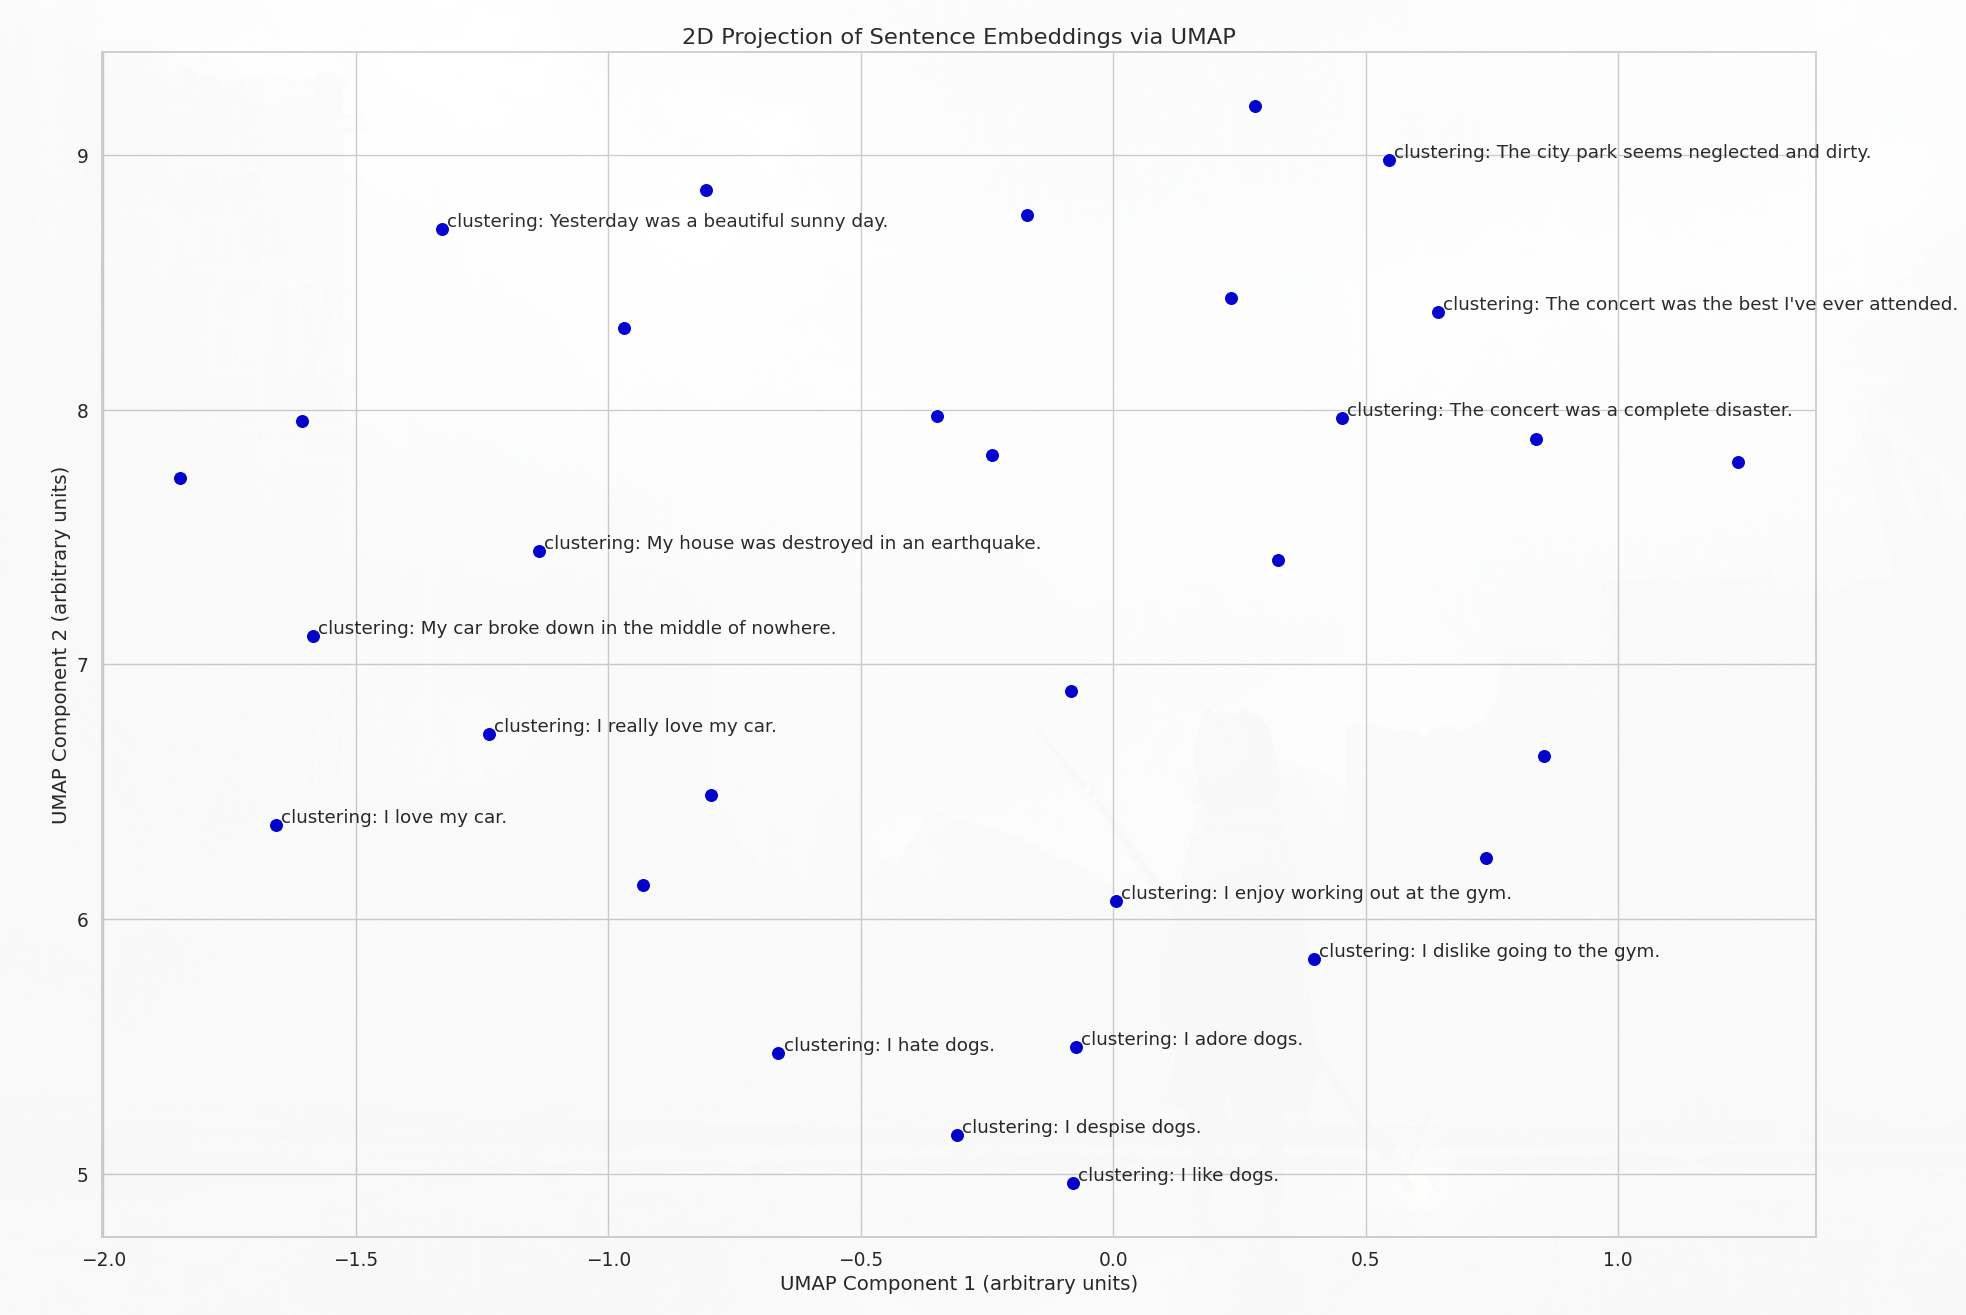
\includegraphics[width=0.95\textwidth]{sentenceEmbeddingExample.png}
    \caption{Example embedding of random sentences generated using OpenAI's ChatGPT o3-mini-high and then performing text embedding using Nomic Text Embedding v1.5 \cite{nussbaum2024nomic}, then projected onto 2 dimensions using UMAP with a random seed of 42, and minimum neighbours of 15. Only some of the labels are for visual clarity.}\label{fig:sentenceEmbeddingExample}
\end{figure}

\subsection{BERT-family Transformers}\label{sec:BERT}
Pre-trained language models (PLMs), such as BERT \cite{devlin2019bert}, have been widely successful in a wide range of NLP tasks through fine-tuning \cite{edunov2019pre, min2023recent}. Fine-tuning is the process of re-training a PLM on specialised tasks, leveraging the model's base knowledge, by applying perturbations to the pre-trained model parameters through gradient descent learning algorithms. These language models, trained on finding an embedding space for natural language as well as stochastically generating tokens to mimic natural language, often provide a great platform to perform task-specific model fine-tuning. 
Platforms such as HuggingFace \cite{wolf2019huggingface}, allow authors to upload these pre-trained model parameters which in-turn allows researchers to download them for them fine-tuning. Moreover, task-specific fine-tuned models parameters are uploaded, downloaded and shared on these platforms. These fine-tuned models are useful for researchers whose focus lies outside of optimising these model parameters.
In this section, we talk about the BERT-family of language models.

\subsubsection{BERT}
The Bidirectional Encoder Representations from Transformer (BERT) language model introduced in 2018 by Google AI Language team in (\citet{devlin2019bert}) was designed to learn deep bidirectional representations from unlabelled text. It achieved this by learning the left and right context in every layer of the model. The model implementation can be split into two phases: \todo{sprinkle some images in here.} (1) the pre-training phase; and (2) the fine-tuning phase. This allows the model architecture to remain common, with many down-stream NLP tasks benefiting from a single PLM. An example illustration can be seen in Figure~\ref{fig:bert1}, where a single model can be fine-tuned on many down-stream tasks by simply replacing the output layer. The model architecture is a multi-layer Transformer encoder based on the original paper (\citet{vaswani2017attention}) which is bidirectional by nature. As the transformer architecture is a very well researched architecture, well represented in the literature and slightly out-of-scope for this paper, we refer the reader to the original paper.

\begin{figure}[htbp]
    \centering
    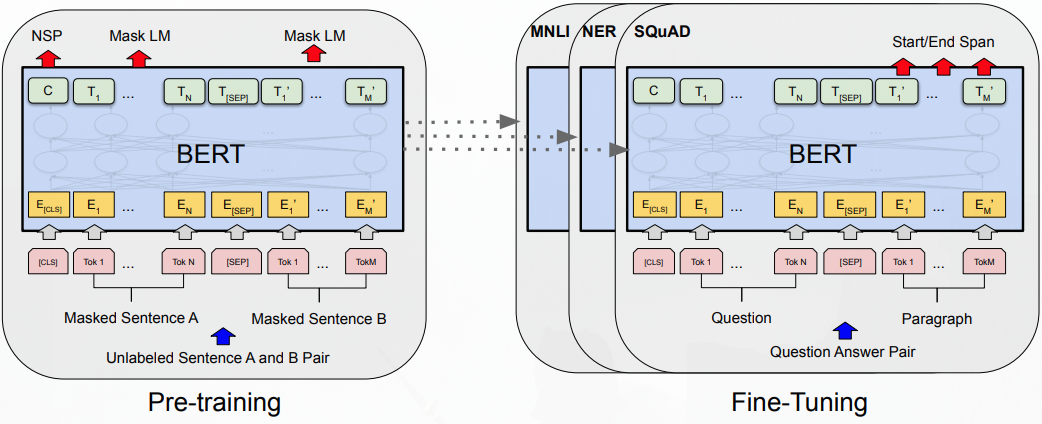
\includegraphics[width=0.95\textwidth]{BERT1.png}
    \caption{The overall pre-training and fine-tuning phases for BERT. For different down-stream tasks, notice the same architecture, except output layer, is used. Source: (\citet{devlin2019bert}).}\label{fig:bert1}
\end{figure}

\textbf{}\\ The pre-training phase can be split into two further training tasks:
\begin{itemize}
    \item  Masked Language Model - During training, a portion of the input tokens are `masked' and the model predicts these masked tokens based on the remaining context, using cross-entropy loss\cite{zhang2018generalized}. In the literature, this is referred to as a Cloze task \cite{taylor1953cloze}. In the experiments conducted by (\citet{devlin2019bert}) 15\% of tokens in each sequence are randomly selected for masking. However, to mitigate the mismatch between pre-training and fine-tuning phases, a training data generator replaces each chosen masked tokens with: (1) the special token \texttt{[MASK]} 80\% of the time; (2) a random token 10\% of the time; and (3) the original token itself 10\% of the time.
    \item Next Sentence Prediction - In this task, the model is trained on a binary classification task prediction the relationship between sentence pairs. Given two sentences \texttt{A} and \texttt{B} either (1) sentence \texttt{B} is the actual sentence that follows \texttt{A} 50\% of the time or (2) sentence \texttt{B} is randomly selected from the corpus 50\% of the time. 
\end{itemize}


\textbf{}\\ The Google AI Language team further fine-tune BERT across 11 NLP tasks, showing that BERT out-performed the state-of-the-art models at its point in time.

As previously mentioned, a benefit of using PLMs such as BERT for NLP tasks (such as text embedding) is the ability to off-load the computationally intensive pre-training and any initial fine-tuning stages to another party. Although, this means that there now exists an implicit trust on that third-party's model parameters. For example, the third-party could be motivated factors to censor certain phrases, artificially injecting testing data into training to increase performance metrics or maliciously change the embedding space. These are all factors which influence our decision on using a PLM and, thus, PLMs with transparently documented data sources, pre-training and fine-tuning should be preferred.

\subsubsection{XLNet and MPNet}
Since the release of the Google AI Language team's BERT, there have been some developments on further improving the performance of PLMs based on BERT's architecture. Namely, we touch on two: XLNet \cite{yang2019xlnet} and MPNet \cite{song2020mpnet}.

One downside of BERT, briefly touched on earlier, is the discrepancy between the pre-training and fine-tuning phases. Although BERT utilises bidirectional context for reconstruction of the special \texttt{[MASK]} token during pre-training, this special token does not exist at the fine-tuning phase. Furthermore, the predicted tokens are masked in the \textit{input} thus BERT assumes the predicted tokens are independent to the surrounding context \cite{yang2019xlnet}. XLNet proposes

\todo[inline, caption={}] {
    \begin{itemize}
        \item Mathematics of BERT (detailed in XLNet paper)
        \item Mathematics of XLNet (detailed in XLNet paper)
        \item Autoregressive vs autoencoder
        \item Architectural changes in XLNet
    \end{itemize}
}


\subsubsection{Nomic}\label{sec:nomic}

\todo[inline, caption={}] {
    \begin{itemize}
        \item Mention nomic is pitched as the first fully reproducable open-source, open-weights, open-data text embedding model
        \item Detail BERT archietcture adaptations
        \item Higher masking rate
        \item AdamW optimiser, learning rate with linear warmup.
        \item (weakly supervised) Pre-training: consistency filtering, curated long context text pairs, gradcache, mixed precision training.
        \item Prefixes on tasks: Symmetric category; asymmetric category.
        \item Supervised contrastive fine-tuning: datasets; learning rate. Randomly sampled mined negatives.
        \item talk about results, especially performance on long context
    \end{itemize}
}


\section{Dimensionality Reduction}\label{sec:dimred}
\todo[inline, caption={}] {
    \begin{itemize}
        \item Talk why dimensionality reduction is needed: visualisation, curse of dimensionality, clustering? Figure out how to structure this well for the story.
        \item Talk about PCA and UMAP.
    \end{itemize}
}
\subsection{PCA}
\todo[inline, caption={}] {
    \begin{itemize}
        \item Talk about PCA mathematics and why its used for dim reduction
        \item Talk about elbowing and finding the most optimal (?)
    \end{itemize}
}

\subsection{UMAP}
\todo[inline, caption={}] {
    \begin{itemize}
        \item Talk about UMAP, the algorithm, the assumptions, the constraints
        \item Use the visualisation of the elephant here.
    \end{itemize}
}

\section{Clustering}

\todo[inline, caption={}] {
    \begin{itemize}
        \item Talk about what clustering does, i.e. looking at trying to categorise or something
        \item Talk about the curse of dimensionality and why clustering does not perform well.
        \item Talk about k-Medoids (supervised), DBSCAN and HDBSCAN (unsupervised).
    \end{itemize}
}

\subsection{k-Medoids}
\todo[inline, caption={}] {
    \begin{itemize}
        \item Talk about algorithm
        \item Talk about the parameters any effects when tuning these parameters.
        \item Talk about drawbacks and benefits of this approach, citations needed.
    \end{itemize}
}
\subsection{DBSCAN}
\todo[inline, caption={}] {
    \begin{itemize}
        \item Talk about algorithm
        \item Talk about the parameters any effects when tuning these parameters.
        \item Talk about drawbacks and benefits of this approach, citations needed.
    \end{itemize}
}
\subsection{HDBSCAN}
\todo[inline, caption={}] {
    \begin{itemize}
        \item Talk about algorithm
        \item Talk about the parameters any effects when tuning these parameters.
        \item Talk about drawbacks and benefits of this approach, citations needed.
    \end{itemize}
}

\section{Clustering Evaluation}

\todo[inline, caption={}] {

    Maybe this should be later on in the methodology? 

    \begin{itemize}
        \item Motivate the need for clustering evaluation.
        \item Just highlight mathematics of each algorithm and mention the need for them.
    \end{itemize}
}
\subsection{Inertia}
\subsection{Silhouette}
\subsection{Davies-Bouldin Index}
\subsection{Calinski-Harabasz Index}

\section{Maybe Optuna}

\chapter{Automatic Label Generation}\label{chap:Methodology}

\section{Data}

The ISIS research facility publish some open-sourced data at (\citet{isisdata}), which contains over 2000 datasets containing instrumentation calibrations and metrics. In addition to this, the ISIS team maintain proprietary, internal datasets that are available on request. Finally, the day-to-day crew additionally maintain an operational log `Operalog' that contains information about faults that occur and remediation steps taken. As mentioned previously, ISIS has an incredibly large number of sensors for instrumentation precision and safety. In the interest of time and research effort, a specialised focus was set on reviewing the ion source component. The ISIS research facility provided us with data logs of the ion source component, with the earliest entry being on the 27$^{th}$ March 2003. In addition to this, we explored the Operalog. \todo{Maybe mention Yuvan?} In the interest of time, this project was divided into two, with this paper focusing on the Operalog. 

\subsection{The Operalog}
The operational log, otherwise referred to as the `Operalog', is an Excel spreadsheet with entries documenting moments of machinery failure within the ISIS facility since 1996 till the end of 2023. Important features are documented in Table~\ref{tab:operalog}. One important point to note is that the day-to-day operational crew have developed custom abbreviations, acronyms and terminology which may not immediately be clear. Additionally, different crew members have varying writing styles and levels of depth of information. Thus, this results in a unstructured text dataset which has a huge variance in quality and quantity of information. Furthermore, as noted in Table~\ref{tab:operalog}, FaultRepair was seemingly made redundant post-2017. Figure~\ref{fig:FaultDescriptionVSFaultRepairs} highlights the distribution in the text lengths of both unstructured text fields. Evidently, FaultRepair has lower quality of information, having most of the entries of less than 10. This is further made clear in the Wordcloud illustrations (Figure~\ref{fig:wc}), where FaultDescription clearly has less free space, meaning it has a larger amount of unique words. This indicates the information extracted from FaultDescription encodes more informative context of the failures that have occurred. Therefore, we only consider the FaultDescription text field.

\rowcolors{2}{gray!10}{white}
\begin{table}[htbp]
    \fontsize{8}{10}\selectfont
    \centering
    \begin{adjustbox}{max width=\textwidth}
    % \begin{tabular}{p{1cm} p{2cm}, p{9cm}}

    \begin{tabular}{p{3cm} p{4cm} p{10cm}}
        \toprule
        \textbf{Feature Name} & \textbf{Data Type} & \textbf{Description} \\
        \midrule
        FaultDate & Date-time & Date the fault occurred, with a precision up to the nearest second. \\
        UserRun & String & Operational cycle that this fault has occurred within. Cycle information up to 2016 can be found at (\citet{isisbeamoperations2024}). \\
        Downtime & Integer & The amount of time, in hours the downtime has occurred for. \\
        Group & String, Fixed Category & The group that the faulty equipment is part of. There are 13 unique equipment groups. \\
        Equipment & String, Fixed Category & The equipment that failed. There are around 200 unique equipment types that have been logged to fail. \\
        FaultDescription & String, Free-form & This is a free-form, unstructured text field that allows the on-shift operational crew to note details about the problem diagnosis and remediation that has occurred. There is no constraint to the size of this text field.\\
        FaultRepair & String, Free-form & Another free-form, unstructured text field that allows the on-shift operational crew to note only the remediation steps. The crew seems to have stopped using this field after the end of 2017, preferring to put remediation steps in FaultDescription. \\
        ManagersComments & String, Free-form & A very rarely used free-form text field, where the manager in charge of the on-shift crew will input comments. \\
        \bottomrule
    \end{tabular}
    \end{adjustbox}
    \caption{\fontsize{9}{10}\selectfont Description of important features (columns) in the Operalog.}
    \label{tab:operalog}
\end{table}

\begin{figure}[htbp]
    \centering
    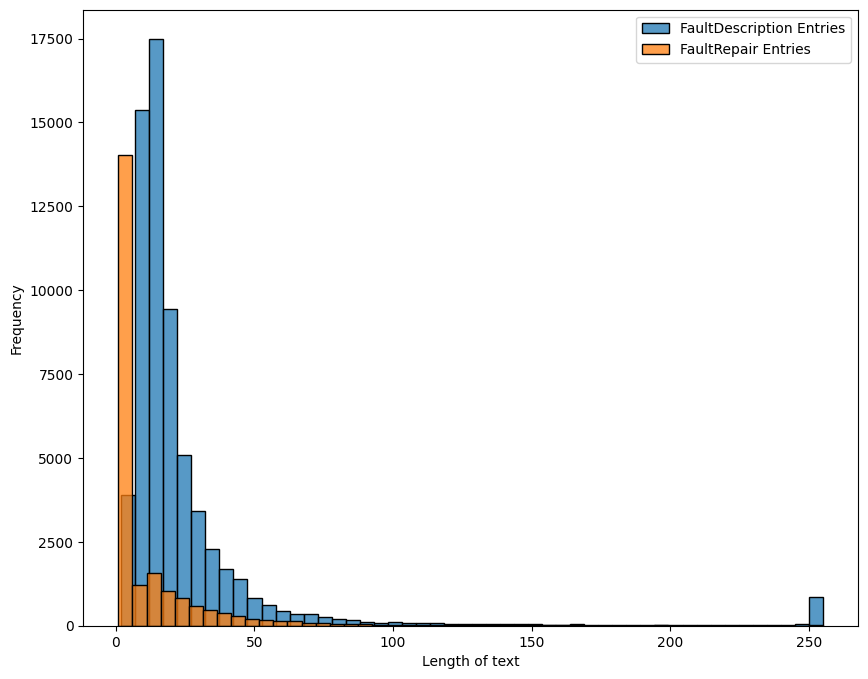
\includegraphics[width=0.7\textwidth]{FaultDescriptionVSFaultRepairs.png}
    \caption{Frequency distribution of the lengths of non-blank text fields FaultDescription and FaultRepair. The bin size is 50, thus bar in the x-axis direction a difference of text length of 10.}\label{fig:FaultDescriptionVSFaultRepairs}
\end{figure}

\begin{figure}[htbp]
    \centering
    \begin{subfigure}[b]{0.48\textwidth}
        \centering
        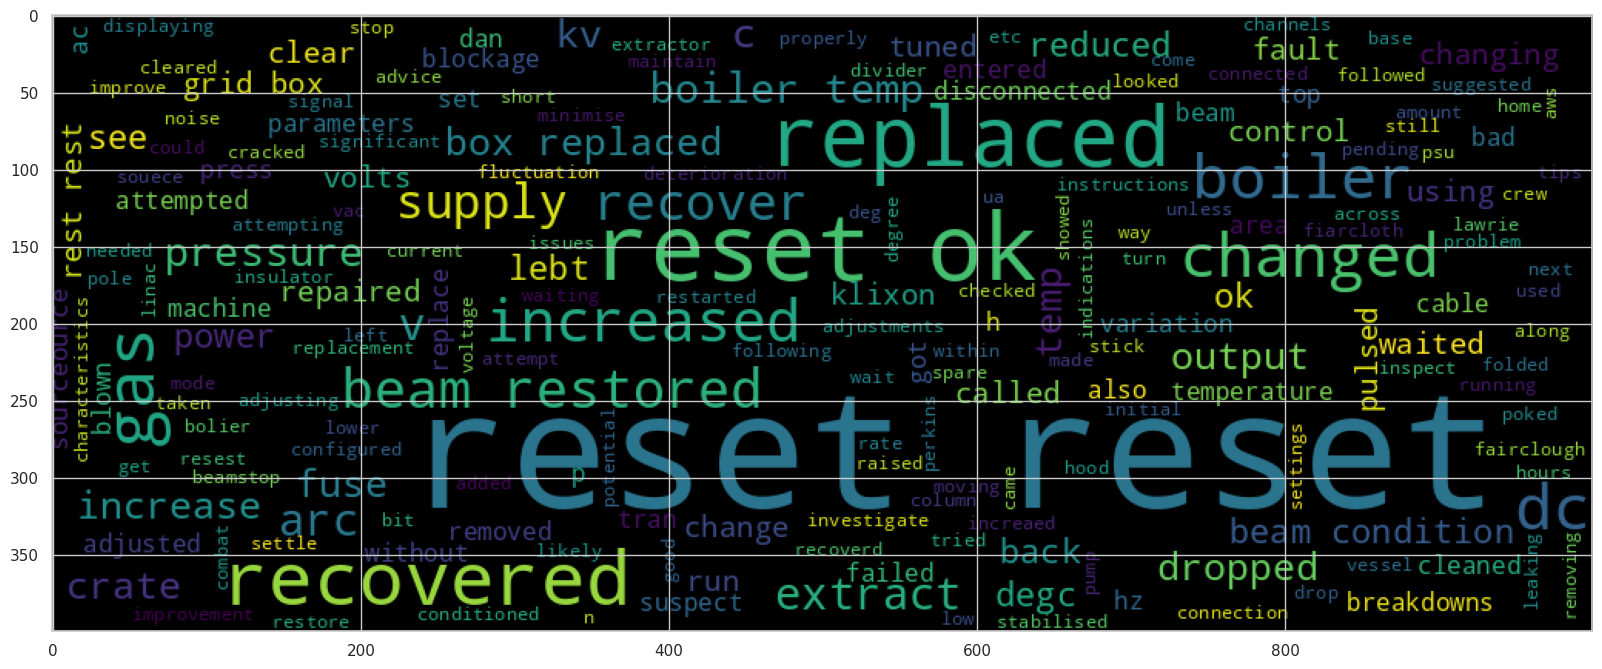
\includegraphics[width=\textwidth]{wcFaultRepairs.png}
        \caption{\fontsize{7}{8}\selectfont FaultRepair}
        \label{fig:wcFaultRepairs}
    \end{subfigure}%
    \hfill
    \begin{subfigure}[b]{0.48\textwidth}
        \centering
        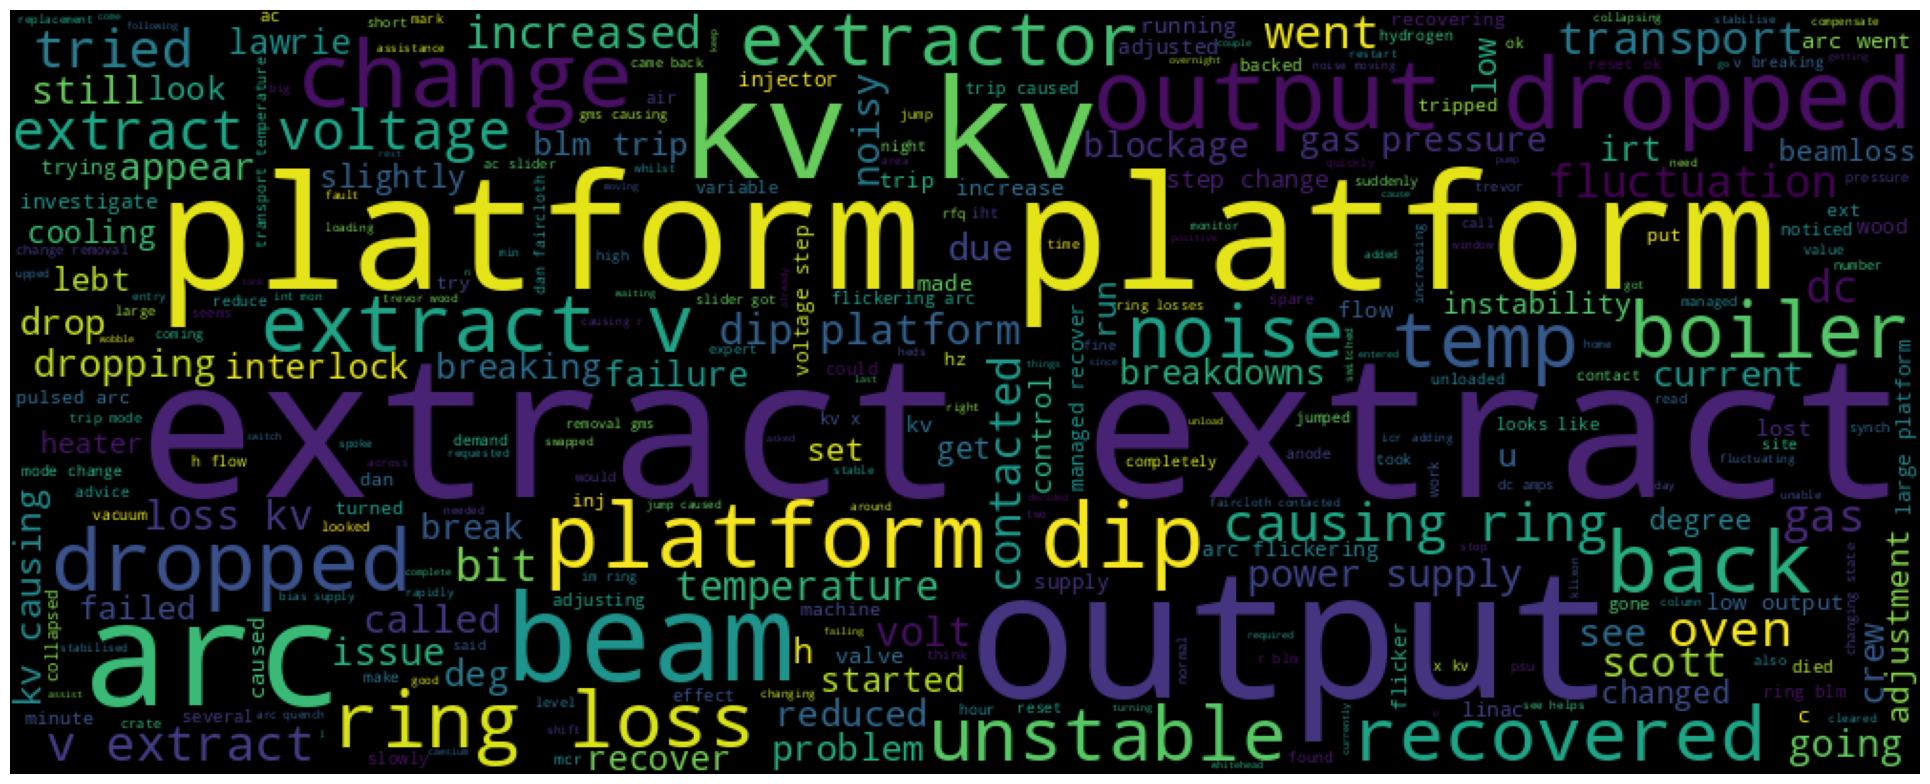
\includegraphics[width=\textwidth]{wcFaultDescription.png}
        \caption{\fontsize{7}{8}\selectfont FaultDescription}
        \label{fig:wcFaultDescription}
    \end{subfigure}
    \caption{Comparison of word clouds for the top 300 most common words for the FaultRepair field versus the FaultDescription field. Larger words are more common, less free space means there more unique words.}
    \label{fig:wc}
\end{figure}





\todo[inline,caption={}]{
    Describe the methods and procedures used.
    The things in this section will include.
    \begin{itemize}
        \item Explaining data format and data visualisation: wordcloud.
        \item Data cleaning steps, including removing key words such as Ion Source.
        \item Text preprocessing steps (cleaning) and computational challenges (tensorflow).
        \item Choosing the best sentence embedding transformer: MPNET, NOMIC.
        \item Data visualisation (before and after sentence embedding): similarity visualisation, explain unique sentences, token length distribution.
        \item Motivate why clustering in higher dimensions performs worse
        \item UMAP, PCA, t-SNE comparison. Motivate using UMAP.
        \item UMAP hyperparameter optimisation.
        \item Performing clustering with kmedoids, dbscan, hdbscan.
        \item Using optuna.
        \item Evaluation of results and choosing the best model (and arguing why hdbscan is the best by looking at the variance of dbscan and inflexibility of kmedoids)
        \item Touch on the production of a CLI application that allows you to mix and match various parts of the pipeline. Motivate the need for command line tool.
    \end{itemize}
}

\chapter{Results and Discussion}

\todo[inline,caption={}]{
Describe the results and analyse the results
\begin{itemize}
    \item Analyse the word cloud.
    \item Analyse the sentence embedding results.
    \item Analyse UMAP vs. PCA vs. t-SNE qualitatively and later quantitatively (compared to the clustering).
    \item Anaylse the UMAP hyperparameter optimisation qualitatively, mention that we use Optuna.
\end{itemize}
}

\chapter{Conclusion}

\todo[inline, caption={}]{
    \begin{itemize}
        \item Definitely talk about clear and transparent PLMs and malicious stuff (see BERT section).
    \end{itemize}
}

% \todo[inline,caption={}]{
% Summarize your findings and suggest areas for future work.
% }

% -------------------------
% References
% -------------------------
% \bibliographystyle{plainnat}

\bibliographystyle{plainnat}
\bibliography{refs}  % Uses the external file refs.bib

\end{document}
